\documentclass[12pt,a4paper]{article}

\sloppy

\setlength{\textwidth}{16cm}
\setlength{\textheight}{24cm}
\addtolength{\hoffset}{-1cm}
\addtolength{\voffset}{-2cm}

\usepackage[utf8]{inputenc}
\usepackage[spanish]{babel}
\usepackage{ae}
\usepackage{graphicx}
\usepackage{placeins}

\usepackage{amsmath,amssymb,amsthm}
\usepackage{multicol, array}

\decimalpoint

\usepackage{sectsty}
%\allsectionsfont{\mdseries \raggedright}
\sectionfont{\fontsize{14}{15}\selectfont}
%\chapterfont{\large\sc\centering}
%\chaptertitlefont{\centering}
\subsectionfont{\fontsize{12}{15}\selectfont}
\subsubsectionfont{\fontsize{12}{15}\selectfont}


\usepackage[T1]{fontenc}
\usepackage{textcomp}
\usepackage[slantedGreek]{mathpazo} %% ver psnfss2e
\usepackage{pifont}
\usepackage{newcent}
\usepackage[small, bf, margin=20pt, tableposition=top]{caption}

\usepackage{fancyhdr}


\setlength{\parskip}{2mm}



\theoremstyle{definition}
\newtheorem{theorem}{Ejercicio N$^o$}

\pagestyle{fancy}
\lhead{Mecánica del Continuo 2023 -  U.N.S.L. \\ Depto. de Física -  Licenciatura en Física}
\rhead{
\includegraphics[width=1cm]{/home/juan/Documentos/Docencia/unsl.jpg} }
\vspace*{0.25cm}
\usepackage{float}

\begin{document}



\begin{center}
{\bf \large Práctico N$^o 4:$ \\
Mecánica del Continuo: \\ Esfuerzo}
\end{center}

\bigskip

\section{Una lista aburrida, pero necesaria}
\begin{itemize}
\item[\textbf{a)}] Defina \textit{esfuerzo}
\item[\textbf{b)}] Defina \textit{estado de esfuerzo}
\item[\textbf{c)}] Enumere propiedades importantes del \textit{tensor de esfuerzos}
\item[\textbf{d)}] Consigne el significado de las componentes del \textit{tensor de esfuerzos} 
\item[\textbf{e)}] Defina esfuerzos principales y planos en los que ocurren.
\item[\textbf{f)}] Defina máximo esfuerzo de corte y planos de acción.
\end{itemize}

\section{Para hacer entre \textit{todes} - Clase TP4}
\subsection*{Muestra gratis 1}
El estado de esfuerzos en un punto de un sólido está dado por:
\begin{center}
$[T] \; = \;
\begin{pmatrix}
6 & 5 & -2\\
5 & 3 & 4\\
-2 & 4 & 9
\end{pmatrix}
MPa
$
\end{center}

\begin{itemize}
\item[\textbf{a)}] ¿cuál es el esfuerzo en el plano cuya normal es $\mathbf{e_1}$?
\item[\textbf{b)}] Discrimine, en el vector de esfuerzo del punto anterior, entre esfuerzo normal y tangencial.
\item[\textbf{c)}] ¿Es posible calcular el \textit{máximo esfuerzo normal} y el plano en el que actúa, definido por el vector normal $\mathbf{n}$? De ser así, hágalo.
\item[\textbf{d)}] Calcule los esfuerzos para $-\mathbf{n}$, es decir, \textit{la otra cara de la moneda}
\end{itemize}

\subsection*{Muestra Gratis 2}
Con el estado de esfuerzos del ejercicio anterior, calcule:
\begin{itemize}
\item[\textbf{a)}] El máximo esfuerzo tangencial y el plano en el que actúa.
\item[\textbf{b)}] El esfuerzo \textit{normal} en el plano del \textit{máximo esfuerzo de corte}
\end{itemize}

\newpage


\section{Ejercicios para usted}
%EJERCICIO 1
 \begin{theorem}
El siguiente tensor representa el estado de esfuezo de un punto en un sólido: 
 
 \begin{center}
$[T] \; = \;
\left(\begin{smallmatrix}
1 & 2 & 3\\
2 & 4 & 5\\
3 & 5 & 0
\end{smallmatrix}\right)
MPa
$
 \end{center}

En cada uno de los planos normales a los vectores unitarios $\mathbf{e_1, e_2, e_3}$, (a) ¿cuál es el esfuerzo normal? y (b) ¿cuál es el esfuerzo tangencial total?

\end{theorem}

\bigskip


%EJERCICIO 2
\begin{theorem}
Considere el siguiente estado de esfuerzos en un sólido:

 \begin{center}
$[T] \; = \;
\left(\begin{smallmatrix}
\alpha x_2 & \beta & 0\\
\beta & 0 & 0\\
0 & 0 & 0
\end{smallmatrix}\right) 
$
 \end{center}
 \noindent donde $\alpha [MPa \; m^{-1}]$  $\beta [MPa] \in \mathbb{R}$ y son positivos.
 \noindent (a) Determine y bosqueje la distribución del vector de esfuerzos que actúa sobre la zona delimitada por $(0,1,1);(0,-1,1);(0,1,-1);(0,-1,-1)$, y es normal a $\mathbf{e_1}$. (b) Determine la fuerza total  y el momento respecto del origen, que actúan sobre el cuadrado del punto anterior.
\end{theorem}

\bigskip
%EJERCICIO 3

\begin{theorem}

Suponga que $\mathbf{{t_{n_1}}}$ y $\mathbf{{t_{n_2}}}$ son vectores esfuerzo actuando en planos $\mathbf{n_1}$ y $\mathbf{n_2}$, ambos en el mismo punto del continuo con un estado de esfuerzos determinado por $\mathbf{T}$.

\noindent a) Probar que la componente de $\mathbf{{t_{n_1}}}$ en $\mathbf{n_2}$ y la componente de $\mathbf{{t_{n_2}}}$ a lo largo de $\mathbf{n_1}$ son iguales si y solo si $\mathbf{T}$ es simétrico.

\noindent b) ¿Cuáles son las condiciones físicas necesarias para que $\mathbf{T}$ sea simétrico?

\noindent c) Resolver el ejercicio 4.29 de la bibliografía Lai 4° Edición.
\end{theorem}

\bigskip

%E 4
\begin{theorem}
Escribir los vectores esfuerzo en \textit{cada una} de las superficies de la Fig. (\ref{fig}) en términos de los valores dados en el gráfico y la base ortonormal $\lbrace \mathbf{e_1},\mathbf{e_2} \rbrace$.


\begin{figure}[H] 
%\begin{center}
\centering 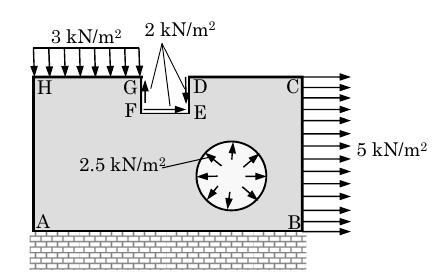
\includegraphics[width=60mm]{ej2}
\caption{Las unidades utilizadas son $kN/m^2=10^3 Pa$} 
\label{fig}
%\end{center}
\end{figure}
\end{theorem}



%E 5
\begin{theorem}

Las componentes de diferentes tensores esfuerzo, respecto de una base $\mathbf{e_i}$, en un punto del continuo (en $MPa$) son:

$[T_1] \; = \;
\left(\begin{matrix}
12 & 9 & 0\\
9 & -12 & 0\\
0 & 0 & 6
\end{matrix}\right)
$
\hspace*{0.5cm}$[T_2] \; = \;
\left( \begin{matrix}
9 & 0 & 12 \\
0 & -25 & 0 \\
12 & 0 & 16 
\end{matrix} \right)
$
\hspace*{0.5cm} 
$[T_3] \; = \;
\left( \begin{matrix}
1 & -3 & \sqrt{2} \\
-3 & 1 & \sqrt{2} \\
\sqrt{2} & -\sqrt{2} & 4 
\end{matrix} \right)
$


\noindent a) Encontrar el vector de esfuerzo en un plano cuyo vector normal es \linebreak $\mathbf{n}\,=\, 2\mathbf{e_1}-2\mathbf{e_2}+\mathbf{e_3}$

\noindent b) La magnitud del vector de esfuerzo y el ángulo entre el vector de esfuerzo y la normal al plano.

\noindent c) La magnitud de la componente tangencial (o de cizalla) del vector de esfuerzo.

\noindent d) Encontrar el máximo esfuerzo de cizalla y el plano en el que actúa, realizando un gráfico que indique la información anterior.
\end{theorem}


\bigskip

%EJERCICIO 6
\begin{theorem}
El estado de esfuerzo tridimensional en el punto (1,1,-2) de un cuerpo respecto de las coordenadas $(x_1,x_2,x_3)$ es:

\hspace*{4cm}$[T] \; = \;
\left( \begin{matrix}
2 & 3.5 & 2.5 \\
3.5 & 0.0 & -1.5 \\
2.5 & -1.5 & 1.0 
\end{matrix} \right) MPa
$


\medskip
a) Determine el la componente normal y tangencial del vector esfuerzo en el punto (1,1,-2) sobre la superficie esférica cuya ecuación es $x_1^2+(x_2-2)^2+x_3^2\:=\:6$.
\end{theorem}


\bigskip

%EJERCICIO 7
\begin{theorem}
Para el estado de esfuerzo del ejercicio anterior:, 

\noindent a) determinar el vector esfuerzo en un plano (que contiene al punto (1,1,-2)) y está definido por los puntos (0,0,0), (2,-1,3) y (-2,0,-1).

\noindent b) determinar la componente normal y la magnitud y dirección de la componente tangencial de dicho vector esfuerzo.
\end{theorem}


\bigskip


%EJERCICIO 8
\begin{theorem}
Dado el siguiente tensor de esfuerzo en un punto $(x_1,x_2,x_3)$ de un continuo:

\hspace*{4cm}$[T] \; = \;
\left( \begin{matrix}
0 & 0 & Ax_2 \\
0 & 0 & -Bx_3 \\
Ax_2 & -Bx_3 & 0 
\end{matrix} \right)
$

donde A y B son constantes. Determinar:

\noindent a) la fuerza de volumen (body forces) necesaria para que el tensor de esfuerzos corresponda con un estado de equilibrio.

\noindent b) Las tres direcciones y valores principales en el punto $x=Be_2+Ae_3$

\noindent c) El esfuerzo de cizalla máximo y el plano donde actúa en el punto $x=Be_2+Ae_3$.

\noindent d) Realizar un gráfico indicando los resultados de los puntos a,b y c.
\end{theorem}


\bigskip

%E 9
\begin{theorem}
Considerar el tensor de esfuerzos:
\begin{center}
$[T] \; = \;
\left( \begin{matrix}
0 & 100 x_1 & -100x_2 \\
100 x_1 & 0 & 0 \\
-100x_2 & 0 & 0 
\end{matrix} \right) MPa \; m^{-1}
$
\end{center}

(a) Calcular las direcciones principales y los autovalores. (b) Encontrar el esfuerzo en un plano que pasa por el punto $1/2,\sqrt{3}/2, 3$ y es tangente a la superficie cilíndrica circular $x_1^2+x_2^2=1$ en ese punto. 


\end{theorem}


\bigskip

%EJERCICIO 10

\begin{theorem} \label{esiete}
Considere un cilindro cuyas paredes están delimitadas por los radios $r_1 = 0.5 m$ y $r_2 = 0.52 m$, como se muestra en la Fig.(\ref{ej7}). Considerando que la presión exterior ($\forall r > r_2$) es la presión atmosférica $p_o = 101325 Pa$ y que la presión interior ($\forall r < r_1$) es $p_i = 10 p_o$:

\noindent a) Calcular el estado de esfuerzo de la pared del cilindro.

\noindent b) Calcular el estado de esfuerzo de la pared del cilindro, utilizando la aproximación de pared delgada.

\noindent c) Comparar mediante una gráfica $T_{\theta \theta}$ vs. $r$ los dos modelos calculados.

\noindent d) Supongamos que la presión interior y la exterior son intercambiadas. Calcular según el modelo del punto \textbf{a} y comparar los resultados de $T_{\theta \theta}$ mediante una gráfica. 

\end{theorem}

\begin{figure}[htb!] 
\begin{center}
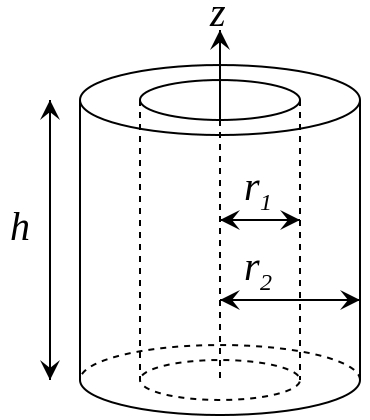
\includegraphics[width=40mm]{cilindro.jpg}
\caption{El cilindro del ejercicio \ref{esiete}.} 
\label{ej7}
\end{center}
\end{figure}


\end{document}

